\documentclass[12pt]{scrartcl}

\usepackage[T1]{fontenc}
\usepackage[utf8]{inputenc}
\usepackage{amsmath}
\usepackage{amsfonts}
\usepackage{amssymb}
\usepackage{amsbsy}
\usepackage{graphicx}
\usepackage{float}
\usepackage{array}
\usepackage{booktabs}
\usepackage{multirow}
\usepackage{bm}
\usepackage{verbatim}
\usepackage[english]{babel}
\usepackage{color}
\usepackage{url}
\usepackage{fancybox}
\usepackage[stable]{footmisc}
\usepackage[format=plain,labelfont=bf]{caption}
\usepackage{fancyhdr}
\usepackage{natbib}
\usepackage{calc}
\usepackage{textcomp}
\usepackage[pdftex,pdfborder={0 0 0}]{hyperref}
\usepackage{pdfpages}
\usepackage{tikz}
\usetikzlibrary{shapes,arrows,decorations.pathmorphing}
\usepackage{amsmath}
\usepackage{easybmat}
\usepackage{multirow,bigdelim}

\renewcommand*{\familydefault}{\sfdefault}
\newcommand*\hexbrace[2]{%
  \underset{#2}{\underbrace{\rule{#1}{0pt}}}}
  
% Margins
\addtolength{\textheight}{1.0cm}
\addtolength{\oddsidemargin}{-0.5cm}
\addtolength{\evensidemargin}{-0.5cm}
\addtolength{\textwidth}{1.0cm}
\parindent=0em

% New math commands
\newcommand{\overbar}[1]{\mkern 1.5mu\overline{\mkern-1.5mu#1\mkern-1.5mu}\mkern 1.5mu}
\DeclareMathOperator{\diag}{diag}
\DeclareMathOperator{\Diag}{Diag}
\DeclareMathOperator{\tr}{tr}
\DeclareMathOperator{\Cov}{Cov}
\DeclareMathOperator{\Cor}{Cor}
\newcommand\independent{\protect\mathpalette{\protect\independenT}{\perp}}
\def\independenT#1#2{\mathrel{\setbox0\hbox{$#1#2$}%
\copy0\kern-\wd0\mkern4mu\box0}} 

% Appropriate font for \mathcal{}
\DeclareSymbolFont{cmmathcal}{OMS}{cmsy}{m}{n}
\DeclareSymbolFontAlphabet{\mathcal}{cmmathcal}

% Set subscript and superscripts positions
\everymath{
\fontdimen13\textfont2=5pt
\fontdimen14\textfont2=5pt
\fontdimen15\textfont2=5pt
\fontdimen16\textfont2=5pt
\fontdimen17\textfont2=5pt
}

% Bibliography style
\setlength{\bibsep}{1pt}

% Part
\renewcommand\partheadstartvskip{\clearpage\null\vfil}
\renewcommand\partheadmidvskip{\par\nobreak\vskip 20pt\thispagestyle{empty}}
\renewcommand\partheadendvskip{\vfil\clearpage}
\renewcommand\raggedpart{\centering}

\begin{document}
\title{Multivariate localization}
\author{Benjamin Ménétrier}
\date{Last update: \today}

\thispagestyle{empty}

\maketitle
\begin{center}
Documentation for the code "BUMP", distributed under the CeCILL-C license.\\
Copyright \copyright 2015-... UCAR, CERFACS, METEO-FRANCE, IRIT and Meteorologisk Institutt
\end{center}

\tableofcontents

\clearpage


\section{Framework}

\subsection{State vector definition}
The state vector $\mathbf{x} \in \mathbb{R}^n$ is split into $Q$ concatenated sub-vectors $\mathbf{x}_q$ (called ``groups''), each one gathering $P_q$ sub-vectors $\mathbf{x}_{p,q}$ of size $n_q$ (called ``variables''). Each sub-vector $\mathbf{x}_{p,q}$ corresponds to the data for a given physical variable (e.g. zonal wind, temperature, humidity, etc.). In a given group, all variables have the same size ($n_q$). Thus:
\begin{align}
\mathbf{x} = \left( \begin{array}{c}
\mathbf{x}_1 \\[1ex]
\hline
\vdots \\
\hline
\mathbf{x}_Q
\end{array} \right) \quad \text{and} \quad \mathbf{x}_q = \left( \begin{array}{c}
\mathbf{x}_{1,q} \\[1ex]
\hline
\vdots \\
\hline
\mathbf{x}_{P_q,q}
\end{array} \right) 
\end{align}
As a consequence:
\begin{itemize}
\item The total number of variables is $\displaystyle P = \sum_{q=1}^Q P_q$.
\item Each group $\mathbf{x}_q$ has a size $P_q n_q$, so the full state vector size is $n = \displaystyle \sum_{q=1}^Q P_q n_q$.
\end{itemize}

\subsection{Illustration setup}
A simple example will be used as an illustration throughout this note. We define a vector $\mathbf{x}$ with $Q = 3$ groups, where $P_1 = 3$, $P_2 = 1$ and $P_3 = 2$:
\begin{align}
\begin{array}{c@{}c}
\mathbf{x} = \left( \begin{array}{c}
\mathbf{x}_{1,1} \\
\mathbf{x}_{2,1} \\
\mathbf{x}_{3,1} \\[1ex]
\hline
\mathbf{x}_{1,2} \\[1ex]
\hline
\mathbf{x}_{1,3} \\
\mathbf{x}_{2,3}
\end{array} \right)
& 
\begin{array}{l}
\\[-8.5mm] \rdelim\}{3}{6mm}[$\mathbf{x}_1$ (1$^\text{st}$ group of variables)] \\[11.5mm] \rdelim\}{1}{6mm}[$\mathbf{x}_2$ (2$^\text{nd}$ group of variables)] \\[3.5mm] \rdelim\}{2}{6mm}[$\mathbf{x}_3$ (3$^\text{rd}$ group of variables)]
\end{array} \\[-1ex]
\end{array}
\end{align}

\subsection{Localization square-root}
The localization matrix $\mathbf{L} \in \mathbb{R}^{n \times n}$ is applied to $\mathbf{x}$. The main issue is to design a positive semi-definite $\mathbf{L}$ matrix, and the simplest solution is to build it as:
\begin{align}
\mathbf{L} = \mathbf{UU}^\textrm{T}
\end{align}
where $\mathbf{U} \in \mathbb{R}^{n \times m}$ is called a ``square-root'' of the localization matrix $\mathbf{L}$. The number of colums $m$ of the square-root $\mathbf{U}$ can be smaller or larger than the number of lines $n$. The control vector $\mathbf{v} \in \mathbb{R}^m$ is such that:
\begin{align}
\mathbf{x} = \mathbf{U} \mathbf{v}
\end{align}
We can define a component $\mathbf{U}_q \in \mathbb{R}^{n_q \times m_q}$ for each group. The relationship between the number of columns $m_q$ of each component $\mathbf{U}_q$ and the total number of columns $m$ of $\mathbf{U}$ depends on the multivariate strategy.\\
$  $\\
The main idea behind this distribution of variables into groups is to apply a localization based on the same component to all the variables pairs within a given group. Thus, the number of distinct component can be reduced if the number of groups is smaller than the number of variables.

\section{Zero cross-localization between groups}
For the first three multivariate strategies, cross-correlations between groups are cut off (i.e. cross-localization is zero). Localization is non-zero only for auto-correlations and cross-correlations between variables of the same group.

\subsection{Univariate localization}
For the case where even cross-correlations between variables of the same group are cut off, the square-root $\mathbf{U}$ can be defined as:
\begin{align}
\mathbf{U} = \left( \begin{array}{ccc|c|cc}
\mathbf{U}_1 & 0 & 0 & 0 & 0 & 0 \\
0 & \mathbf{U}_1 & 0 & 0 & 0 & 0 \\
0 & 0 & \mathbf{U}_1 & 0 & 0 & 0 \\[0.3ex]
\hline
0 & 0 & 0 & \mathbf{U}_2 & 0 & 0 \\[0.3ex]
\hline
0 & 0 & 0 & 0 & \mathbf{U}_3 & 0 \\
0 & 0 & 0 & 0 & 0 & \mathbf{U}_3
\end{array} \right)
\end{align}
Thus:
\begin{align}
\mathbf{L} = \left( \begin{array}{ccc|c|cc}
\mathbf{U}_1 \mathbf{U}_1^\mathrm{T} & 0 & 0 & 0 & 0 & 0 \\
0 & \mathbf{U}_1 \mathbf{U}_1^\mathrm{T} & 0 & 0 & 0 & 0 \\
0 & 0 & \mathbf{U}_1 \mathbf{U}_1^\mathrm{T} & 0 & 0 & 0 \\[0.3ex]
\hline
0 & 0 & 0 & \mathbf{U}_2 \mathbf{U}_2^\mathrm{T} & 0 & 0 \\[0.3ex]
\hline
0 & 0 & 0 & 0 & \mathbf{U}_3 \mathbf{U}_3^\mathrm{T} & 0 \\
0 & 0 & 0 & 0 & 0 & \mathbf{U}_3 \mathbf{U}_3^\mathrm{T}
\end{array} \right)
\end{align}
In this case, the total control vector size is $\displaystyle m = \sum_{q=1}^Q P_q m_q$

\subsection{Duplicated localization}
It is possible to define the cross-localization between the variables of a same group as duplicates of the diagonal localization, by defining $\mathbf{U}$ as: 
\begin{align}
\mathbf{U} & = \left( \begin{array}{c|c|c}
\mathbf{U}_1 & 0 & 0 \\
\mathbf{U}_1 & 0 & 0 \\
\mathbf{U}_1 & 0 & 0 \\[0.3ex]
\hline
0 & \mathbf{U}_2 & 0 \\[0.3ex]
\hline
0 & 0 & \mathbf{U}_3 \\
0 & 0 & \mathbf{U}_3
\end{array} \right) \nonumber \\
& = \left( \begin{array}{c|c|c}
\mathbf{I}_1 & 0 & 0 \\
\mathbf{I}_1 & 0 & 0 \\
\mathbf{I}_1 & 0 & 0 \\[0.3ex]
\hline
0 & \mathbf{I}_2 & 0 \\[0.3ex]
\hline
0 & 0 & \mathbf{I}_3 \\
0 & 0 & \mathbf{I}_3
\end{array} \right)
\left( \begin{array}{c|c|c}
\mathbf{U}_1 & 0 & 0 \\[0.3ex]
\hline
0 & \mathbf{U}_2 & 0 \\[0.3ex]
\hline
0 & 0 & \mathbf{U}_3
\end{array} \right)
\end{align}
where $\mathbf{I}_q \in \mathbf{R}^{n_q,n_q}$ is the identity matrix of size $n_q$. Thus:
\begin{align}
\mathbf{L} = \left( \begin{array}{ccc|c|cc}
\mathbf{U}_1 \mathbf{U}_1^\mathrm{T} & \mathbf{U}_1 \mathbf{U}_1^\mathrm{T} & \mathbf{U}_1 \mathbf{U}_1^\mathrm{T} & 0 & 0 & 0 \\
\mathbf{U}_1 \mathbf{U}_1^\mathrm{T} & \mathbf{U}_1 \mathbf{U}_1^\mathrm{T} & \mathbf{U}_1 \mathbf{U}_1^\mathrm{T} & 0 & 0 & 0 \\
\mathbf{U}_1 \mathbf{U}_1^\mathrm{T} & \mathbf{U}_1 \mathbf{U}_1^\mathrm{T} & \mathbf{U}_1 \mathbf{U}_1^\mathrm{T} & 0 & 0 & 0 \\[0.3ex]
\hline
0 & 0 & 0 & \mathbf{U}_2 \mathbf{U}_2^\mathrm{T} & 0 & 0 \\[0.3ex]
\hline
0 & 0 & 0 & 0 & \mathbf{U}_3 \mathbf{U}_3^\mathrm{T} & \mathbf{U}_3 \mathbf{U}_3^\mathrm{T} \\
0 & 0 & 0 & 0 & \mathbf{U}_3 \mathbf{U}_3^\mathrm{T} & \mathbf{U}_3 \mathbf{U}_3^\mathrm{T}
\end{array} \right)
\end{align}*
In this case, the total control vector size is $\displaystyle m = \sum_{q=1}^Q m_q$

\subsection{Duplicated and weighted localization}
A variant of the previous case uses group-specific lower triangular matrices $\mathbf{S}^q \in \mathbb{R}^{P_q \times P_q}$ to define $\mathbf{U}$ as: 
\begin{align}
\mathbf{U} & = \left( \begin{array}{ccc|c|ccc}
S^1_{1,1} \mathbf{U}_1 & 0 & 0 & 0 & 0 & 0 \\
S^1_{2,1} \mathbf{U}_1 & S^1_{2,2} \mathbf{U}_1 & 0 & 0 & 0 & 0 \\
S^1_{3,1} \mathbf{U}_1 & S^1_{3,2} \mathbf{U}_1 & S^1_{3,3} \mathbf{U}_1 & 0 & 0 & 0 \\
\hline
0 & 0 & 0 & S^2_{1,1} \mathbf{U}_2 & 0 & 0 \\[0.3ex]
\hline
0 & 0 & 0 & 0 & S^3_{1,1} \mathbf{U}_3 & 0 \\
0 & 0 & 0 & 0 & S^3_{2,1} \mathbf{U}_3 & S^3_{2,2} \mathbf{U}_3
\end{array} \right) \nonumber \\
& = \left( \begin{array}{ccc|c|ccc}
S^1_{1,1} \mathbf{I}_1 & 0 & 0 & 0 & 0 & 0 \\
S^1_{2,1} \mathbf{I}_1 & S^1_{2,2} \mathbf{I}_1 & 0 & 0 & 0 & 0 \\
S^1_{3,1} \mathbf{I}_1 & S^1_{3,2} \mathbf{I}_1 & S^1_{3,3} \mathbf{I}_1 & 0 & 0 & 0 \\
\hline
0 & 0 & 0 & S^2_{1,1} \mathbf{I}_2 & 0 & 0 \\[0.3ex]
\hline
0 & 0 & 0 & 0 & S^3_{1,1} \mathbf{I}_3 & 0 \\
0 & 0 & 0 & 0 & S^3_{2,1} \mathbf{I}_3 & S^3_{2,2} \mathbf{I}_3
\end{array} \right) \left( \begin{array}{ccc|c|cc}
\mathbf{U}_1 & 0 & 0 & 0 & 0 & 0 \\
0 & \mathbf{U}_1 & 0 & 0 & 0 & 0 \\
0 & 0 & \mathbf{U}_1 & 0 & 0 & 0 \\[0.3ex]
\hline
0 & 0 & 0 & \mathbf{U}_2 & 0 & 0 \\[0.3ex]
\hline
0 & 0 & 0 & 0 & \mathbf{U}_3 & 0 \\
0 & 0 & 0 & 0 & 0 & \mathbf{U}_3
\end{array} \right)
\end{align}
Thus:
\begin{align}
\mathbf{L} = \left( \begin{array}{ccc|c|cc}
W^1_{1,1} \mathbf{U}_1 \mathbf{U}_1^\mathrm{T} & W^1_{1,2} \mathbf{U}_1 \mathbf{U}_1^\mathrm{T} & W^1_{1,3} \mathbf{U}_1 \mathbf{U}_1^\mathrm{T} & 0 & 0 & 0 \\
W^1_{2,1} \mathbf{U}_1 \mathbf{U}_1^\mathrm{T} & W^1_{2,2} \mathbf{U}_1 \mathbf{U}_1^\mathrm{T} & W^1_{2,3} \mathbf{U}_1 \mathbf{U}_1^\mathrm{T} & 0 & 0 & 0 \\
W^1_{3,1} \mathbf{U}_1 \mathbf{U}_1^\mathrm{T} & W^1_{3,2} \mathbf{U}_1 \mathbf{U}_1^\mathrm{T} & W^1_{3,3} \mathbf{U}_1 \mathbf{U}_1^\mathrm{T} & 0 & 0 & 0 \\[0.3ex]
\hline
0 & 0 & 0 & W^2_{1,1} \mathbf{U}_2 \mathbf{U}_2^\mathrm{T} & 0 & 0 \\[0.3ex]
\hline
0 & 0 & 0 & 0 & W^3_{1,1} \mathbf{U}_3 \mathbf{U}_3^\mathrm{T} & W^3_{1,2} \mathbf{U}_3 \mathbf{U}_3^\mathrm{T} \\
0 & 0 & 0 & 0 & W^3_{2,1} \mathbf{U}_3 \mathbf{U}_3^\mathrm{T} & W^3_{2,2} \mathbf{U}_3 \mathbf{U}_3^\mathrm{T}
\end{array} \right)
\end{align}
where $\mathbf{W}^q = \mathbf{S}^q \mathbf{S}^{q\mathrm{T}}$ provides the weights applied to each covariance between variables within the group $q$. In practice, it is easier to set $\mathbf{W}^q$ and to compute $\mathbf{S}^q$ using a Cholesky decomposition. It also seems reasonable to set the diagonal elements of $\mathbf{W}^q$ to one.\\
$  $\\
In this case, the total control vector size is $\displaystyle m = \sum_{q=1}^Q P_q m_q$

\section{Implicit cross-localization between groups}
For the last multivariate strategy, cross-correlations between groups are defined implicitly as the product of components of both groups.

\subsection{Crossed localization}
In this case, $\mathbf{U}$ is reduced to a column:
\begin{align}
\mathbf{U} & = \left( \begin{array}{c}
\mathbf{U}_1 \\
\mathbf{U}_1 \\
\mathbf{U}_1 \\[0.3ex]
\hline
\mathbf{U}_2 \\[0.3ex]
\hline
\mathbf{U}_3 \\
\mathbf{U}_3
\end{array} \right) \nonumber \\
& = \left( \begin{array}{c|c|c}
\mathbf{I}_1 & 0 & 0 \\
\mathbf{I}_1 & 0 & 0 \\
\mathbf{I}_1 & 0 & 0 \\[0.3ex]
\hline
0 & \mathbf{I}_2 & 0 \\[0.3ex]
\hline
0 & 0 & \mathbf{I}_3 \\
0 & 0 & \mathbf{I}_3
\end{array} \right)
\left( \begin{array}{c}
\mathbf{U}_1 \\[0.3ex]
\hline
\mathbf{U}_2 \\[0.3ex]
\hline
\mathbf{U}_3
\end{array} \right)
\end{align}
An additional assumption is required here: the components $\mathbf{U}_q$ must all have the same number of columns: $m_1 = ... = m_Q = \overbar{m}$. Thus:
\begin{align}
\mathbf{L} = \left( \begin{array}{ccc|c|cc}
\mathbf{U}_1 \mathbf{U}_1^\mathrm{T} & \mathbf{U}_1 \mathbf{U}_1^\mathrm{T} & \mathbf{U}_1 \mathbf{U}_1^\mathrm{T} & \mathbf{U}_1 \mathbf{U}_2^\mathrm{T} & \mathbf{U}_1 \mathbf{U}_3^\mathrm{T} & \mathbf{U}_1 \mathbf{U}_3^\mathrm{T} \\
\mathbf{U}_1 \mathbf{U}_1^\mathrm{T} & \mathbf{U}_1 \mathbf{U}_1^\mathrm{T} & \mathbf{U}_1 \mathbf{U}_1^\mathrm{T} & \mathbf{U}_1 \mathbf{U}_2^\mathrm{T} & \mathbf{U}_1 \mathbf{U}_3^\mathrm{T} & \mathbf{U}_1 \mathbf{U}_3^\mathrm{T} \\
\mathbf{U}_1 \mathbf{U}_1^\mathrm{T} & \mathbf{U}_1 \mathbf{U}_1^\mathrm{T} & \mathbf{U}_1 \mathbf{U}_1^\mathrm{T} & \mathbf{U}_1 \mathbf{U}_2^\mathrm{T} & \mathbf{U}_1 \mathbf{U}_3^\mathrm{T} & \mathbf{U}_1 \mathbf{U}_3^\mathrm{T} \\[0.3ex]
\hline
\mathbf{U}_2 \mathbf{U}_1^\mathrm{T} & \mathbf{U}_2 \mathbf{U}_1^\mathrm{T} & \mathbf{U}_2 \mathbf{U}_1^\mathrm{T} & \mathbf{U}_2 \mathbf{U}_2^\mathrm{T} & \mathbf{U}_2 \mathbf{U}_3^\mathrm{T} & \mathbf{U}_2 \mathbf{U}_3^\mathrm{T} \\[0.3ex]
\hline
\mathbf{U}_3 \mathbf{U}_1^\mathrm{T} & \mathbf{U}_3 \mathbf{U}_1^\mathrm{T} & \mathbf{U}_3 \mathbf{U}_1^\mathrm{T} & \mathbf{U}_3 \mathbf{U}_2^\mathrm{T} & \mathbf{U}_3 \mathbf{U}_3^\mathrm{T} & \mathbf{U}_3 \mathbf{U}_3^\mathrm{T} \\
\mathbf{U}_3 \mathbf{U}_1^\mathrm{T} & \mathbf{U}_3 \mathbf{U}_1^\mathrm{T} & \mathbf{U}_3 \mathbf{U}_1^\mathrm{T} & \mathbf{U}_3 \mathbf{U}_2^\mathrm{T} & \mathbf{U}_3 \mathbf{U}_3^\mathrm{T} & \mathbf{U}_3 \mathbf{U}_3^\mathrm{T}
\end{array} \right)
\end{align}
In this case, the total control vector size is $\displaystyle m = \overbar{m}$.\\

\subsection{Cross-localization amplitude}
The amplitude of cross-localization is not one in this case. For $1 \le q,q' \le Q$, we denote $\mathbf{u}$ the k$^\textrm{th}$ column of $\mathbf{U}_q$ and $\mathbf{u}'$ the k$^\textrm{th}$ column of $\mathbf{U}_{q'}$. The k$^\textrm{th}$ diagonal coefficient of $\mathbf{U}_q \mathbf{U}_{q'}^\mathrm{T}$ is given by $\langle \mathbf{u},\mathbf{u}' \rangle$, where $\langle \cdot, \cdot \rangle$ denotes the canonical inner product. The Cauchy-Schwartz inequality requires that:
\begin{align}
\vert \langle \mathbf{u},\mathbf{u}' \rangle \vert & \le \sqrt{\langle \mathbf{u},\mathbf{u} \rangle \langle \mathbf{u}',\mathbf{u}' \rangle}
\end{align}
Thus, the cross-localization amplitude between groups $q$ and $q'$ is necessarily smaller than the geometric mean of the auto-localization amplitudes for groups $q$ and $q'$. Besides, the more the vectors $\mathbf{u}$ and $\mathbf{u}'$ have different shapes, the smaller their inner product and the smaller the cross-localization amplitude.
\begin{center}
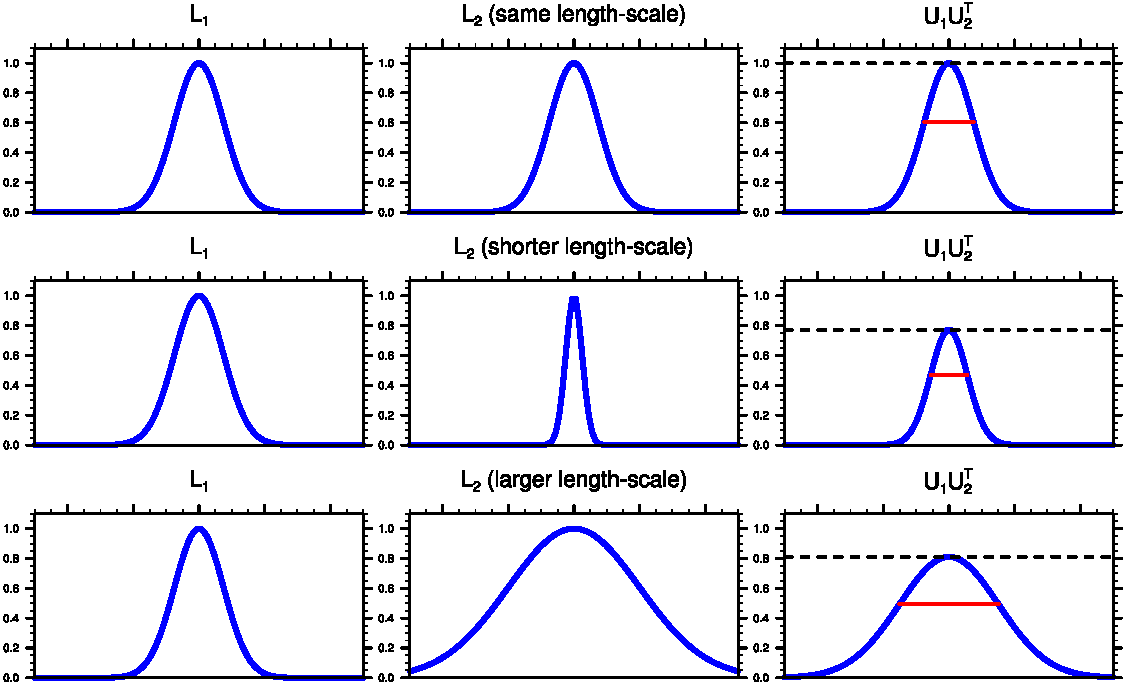
\includegraphics[width=\linewidth]{convolution_exp.pdf}
\captionof{figure}{1D illustration of the product of two localization square-root, with Gaussian localization functions. The dashed black line shows the function amplitude, while the solid red line shows the function length-scale.}
\end{center}

\subsection{Mixing 3D and 2D variables}
In many applications, the state vector contains both 3D and 2D variables. To use the crossed method in this case, it is necessary to consider the 2D variables as 3D variables with only one level containing meaningful data (the first or the last level in general) and the other levels set to zero.\\
$  $\\
For sake of simplicity, we assume here that group 1 contains one 3D variable and group 2 contains one 2D variable. We also assume that both control variable $\mathbf{x}$ and control vector $\mathbf{v}$ can be split into $K$ components, each one handling one vertical level:
\begin{align}
\mathbf{x} = \left( \begin{array}{c}
\mathbf{x}_{1,k=1} \\[1ex]
\vdots \\
\mathbf{x}_{1,k=K} \\[1ex]
\hline
\mathbf{x}_{2}
\end{array} \right) \ \text{ and } \ \mathbf{v} = \left( \begin{array}{c}
\mathbf{v}_{k=1} \\[1ex]
\vdots \\
\mathbf{v}_{k=K} \\[1ex]
\end{array} \right)
\end{align}
We can define an extended control variable:
\begin{align}
\mathbf{x}' = \left( \begin{array}{c}
\mathbf{x}_{1,k=1} \\[1ex]
\vdots \\
\mathbf{x}_{1,k=K} \\[1ex]
\hline
\mathbf{x}'_{2,k=1} \\[1ex]
\vdots \\
\mathbf{x}'_{2,k=K} \\[1ex]
\end{array} \right) = \mathbf{E} \mathbf{x}
\end{align}
where $\mathbf{E}$ is the extension operator padding with zeros, so that both sub-vectors have the same size. In general:
\begin{itemize}
\item either $\mathbf{x}'_{2,k=1} = \mathbf{x}_2$ and 
$\mathbf{x}'_{2,k=2}$ to $\mathbf{x}'_{2,k=K}$ are set to zero,
\item or $\mathbf{x}'_{2,k=K} = \mathbf{x}_2$ and 
$\mathbf{x}'_{2,k=1}$ to $\mathbf{x}'_{2,k=K-1}$ are set to zero.
\end{itemize}
The adjoint of $\mathbf{E}$, denoted $\mathbf{E}^\mathrm{T}$, is thus a reduction operator removing the zeroed levels from the extended control variable $\mathbf{x}'$ to yield the control variable $\mathbf{x}$:
\begin{align}
\mathbf{x} = \mathbf{E}^\mathrm{T} \mathbf{E} \mathbf{x}
\end{align}
We define an extended square-root $\mathbf{U}'_2$:
\begin{align}
\mathbf{U}'_2 = \left( \begin{array}{cccc}
\mathbf{U}_2 & 0 & \dots & 0 \\[1ex]
0 & 0 & \dots & 0 \\
\vdots & \vdots & \ddots & \vdots \\
0 & 0 & \dots & 0
\end{array} \right) \ \text{ or } \ \mathbf{U}'_2 = \left( \begin{array}{cccc}
0 & \dots & 0 & 0\\
\vdots & \ddots & \vdots & \vdots\\
0 & \dots & 0 & 0 \\
0 & \dots & 0 & \mathbf{U}_2
\end{array} \right)
\end{align}
depending on the location of the 2D level in the 3D grid, at level 1 or $K$, respectively. The extended square-root $\mathbf{U}$ is then given by:
\begin{align}
\mathbf{U}' = \left( \begin{array}{c}
\mathbf{U}_1 \\[1ex]
\hline
\mathbf{U}'_2 \\[1ex]
\end{array} \right)
\end{align}
Finally, we get
\begin{align}
\mathbf{x}' = \mathbf{U}' \mathbf{v}
\end{align}
so we can conclude that:
\begin{align}
\mathbf{U} = \mathbf{E}^\mathrm{T} \mathbf{U}'
\end{align}
In practice, the operator $\mathbf{E}^\mathrm{T} \mathbf{U}'$ can be optimized to avoid the storage in memory of the extended variable $\mathbf{x}'$, keeping  the relevant level only for the 2D variables.

\bibliographystyle{mybib-en}
\bibliography{multivariate_localization}
\end{document}
